\title{DBIx::Class Training}
\author{Stefan Hornburg (Racke), Peter Mottram (SysPete)}
\date{Perl Dancer Conference 2015, Vienna, 20th October 2015}

\begin{document}
\maketitle

\input sponsors.tex

\begin{frame}
  \titlepage
\end{frame}

\cleardoublepage

\tableofcontents

\cleardoublepage

\section{Introduction}

This training describes a sample application making use of
DBIx::Class and additional modules which makes you life
way easier. So first of all, we give you an idea what
the application is about.

\subsection{TravelDance Application}

You enjoy traveling, don't you? Even if not, we take you
along for a ride.

\begin{frame}{Traveling is Fun}
% https://pixabay.com/en/volkswagen-car-bus-mobile-home-158463/
\begin{figure}[!ht]
\centering

\includegraphics[width=1\linewidth]{img/volkswagen.png}
\end{figure}
\end{frame}

\subsubsection{Countries}

You can take this to another level, like doing a
competition between who visited the most countries:

% All images downloaded from Wikipedia

\begin{frame}{Countries}
\begin{figure}[!ht]
\centering

\begin{minipage}{.24\textwidth}
\centering

\includegraphics[width=1\linewidth]{img/countries/canada.png}
\caption{Canada}
\end{minipage}
% avoid paragraph break
\begin{minipage}{.24\textwidth}
\centering

\includegraphics[width=0.8\linewidth]{img/countries/austria.png}
\caption{Austria}
\end{minipage}
% avoid paragraph break
\begin{minipage}{.24\textwidth}
\centering

\includegraphics[width=0.8\linewidth]{img/countries/slovakia.png}
\caption{Slovakia}
\end{minipage}
% avoid paragraph break
\begin{minipage}{.24\textwidth}
\centering

\includegraphics[width=0.8\linewidth]{img/countries/usa.png}
\caption{USA}
\end{minipage}

\end{figure}

\end{frame}

\subsubsection{Topics of Application}

\begin{frame}{Topics of Application}
\begin{itemize}
\item Countries
\item Users
\item Locations
\end{itemize}
\end{frame}

Locations include the country and the date when the 
user visited it:

\begin{frame}{Locations}
\begin{itemize}
\item Country
\item User
\item Visited date
\item ...
\end{itemize}
\end{frame}

Of course there are already applications around to manage
your travel destinations.

%\note{
%I'm currently using TripAdvisor's app.
%}

\begin{frame}{Existing Applications}
\begin{itemize}
\item \sout{Privacy}
\item \sout{Options}
\item Slow ?
\end{itemize}
\end{frame}

\begin{frame}{Our Application}
\begin{itemize}
\item Fast
\item Privacy
\item Options
\end{itemize}
\end{frame}

\subsection{Database}
\begin{frame}{Database}
\centering
We need a database ...
\end{frame}

... something like that.

\begin{frame}{Database}
% https://pixabay.com/en/bottles-empty-glass-container-392689/
\begin{figure}[!ht]
\centering
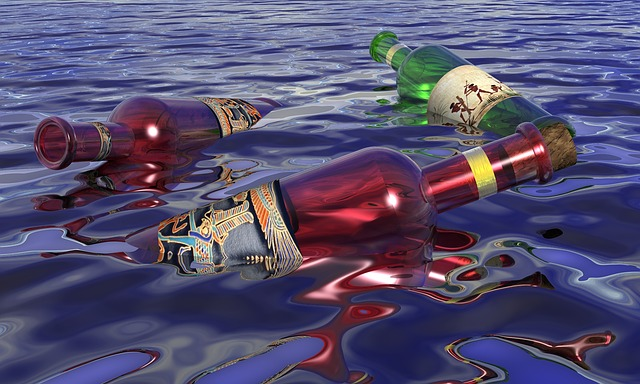
\includegraphics[width=0.8\linewidth]{img/bottles.jpg}
\end{figure}
\end{frame}

Seriously, we are going to use a SQL database like
PostgreSQL:

\begin{frame}{Database}
% https://en.wikipedia.org/wiki/PostgreSQL#/media/File:Postgresql_elephant.svg
\begin{figure}[!ht]
\centering

\includegraphics[width=0.4\linewidth]{img/postgresql.png}
\caption{"Postgresql elephant" by Jeff MacDonald}
\end{figure}
\end{frame}

\begin{frame}{SQL is ...}
\begin{itemize}
\item SQL is ... boring
\item SQL is ... complex
\item SQL is ... incompatible
\item SQL is ... not object oriented
\end{itemize}
\end{frame}

%\begin{frame}{Complex SQL query}
% add example for complex SQL query
%\end{frame}

Just for the fun it, later you will learn how do you
use DBIx::Class to retrieve hash references instead of
objects!

\begin{frame}{DBIx::Class to the rescue!}
\centering
DBIx::Class is a
\begin{description}
\item[ORM] Object Relationship Manager
\end{description}
\end{frame}

\begin{frame}{Business Logic}
% move business logic into schema
\end{frame}

\begin{frame}{Life Savers for DBIx::Class}
% https://pixabay.com/en/candy-cane-candy-cane-winter-488009/
\begin{figure}[!ht]
\centering

\includegraphics[width=0.8\linewidth]{img/candy-cane.jpg}
\end{figure}
\end{frame}

\subsection{Starting with DBIx::Class}

\begin{frame}{Starting with DBIx::Class}
\begin{itemize}
\item Existing project
\item New project
\end{itemize}
\end{frame}

\subsubsection{Existing Project}

You can use \verb|dbicdump| to create a ``boilerplate'' schema from the
existing database.

\begin{frame}[fragile]{dbicdump}
\begin{lstlisting}
dbicdump -o dump_directory=/home/dance/TravelDance/lib 
         TravelDance::Schema 
         dbi:Pg:dbname=perldance
\end{lstlisting}
\end{frame}

\verb|dbicdump| also provides additional options, e.g.
including \verb|DBIx::Class| components, which we cover
later in the training.

\begin{frame}[fragile]{dbicdump with Components}
\begin{lstlisting}
dbicdump -o dump_directory=/home/dance/TravelDance/lib 
         -o components='["InflateColumn::DateTime"]'
         TravelDance::Schema 
         dbi:Pg:dbname=perldance
\end{lstlisting}
\end{frame}

\subsubsection{Creating database}
Starting a new project involves creating a database, which
isn't as simple as you would think.

MySQL databases should be created with UTF8 encoding and appropriate 
collation for your local, for example:

\begin{frame}[fragile]{Creating MySQL database}
\begin{lstlisting}
    CREATE DATABASE "my_shop_db"
        DEFAULT CHARACTER SET utf8
        DEFAULT COLLATE utf8_general_ci;
\end{lstlisting}
\end{frame}

The following L<Connection attributes|DBIx::Class::Storage::DBI/DBIx::Class specific connection attributes> are recommended as a minimum for MySQL:

\begin{frame}[fragile]{MySQL Connection attributes}
\begin{lstlisting}
    mysql_enable_utf8 => 1,
    set_strict_mode => 1,
\end{lstlisting}
\end{frame}

NOTE: we no longer recommend the use of 
\verb|on_connect_call =>'set_strict_mode'| since that also forces MySQL's 
\href{https://dev.mysql.com/doc/refman/5.0/en/sql-mode.html#sqlmode\_only\_full\_group\_by}{ONLY\_FULL\_GROUP\_BY} mode which prevents us from using GROUP BY on PK columns which is a great performance boost for PostgreSQL.

=head1 PostgreSQL

PostgreSQL databases should be created with UT8 encoding, for example:

\begin{frame}[fragile]{Creating PostgreSQL database}
\begin{lstlisting}
    createdb -E UTF8 my_shop_db
\end{lstlisting}
\end{frame}

The following L<Connection attributes|DBIx::Class::Storage::DBI/DBIx::Class specific connection attributes> are recommended as a minimum for PostgreSQL:

\begin{frame}[fragile]{PostgreSQL Connection attributes}
\begin{lstlisting}
    pg_enable_utf8 => 1,
    on_connect_do  => 'SET client_min_messages=WARNING;',
\end{lstlisting}
\end{frame}

\subsubsection{New Project}

For new projects we recommend to write the schema first.

\begin{frame}[fragile]{New Project}
Write Schema first
\end{frame}

\subsection{Exercise I: dbicdump}
\begin{frame}[fragile]{dbicdump Exercise}
\begin{lstlisting}
# clone training repository
git clone \
    git@github.com:interchange/DBIx-Class-Training.git
cd DBIx-Class-Training

# deploy Sqlite database
cd TravelDance
./bin/db-deploy

# explore
sqlite3 traveldance.db
\end{lstlisting}
\end{frame}

\begin{frame}[fragile]{dbicdump Exercise: Explore Database}
\begin{lstlisting}
$ sqlite3 traveldance.db
SQLite version 3.8.11.1 2015-07-29 20:00:57
Enter ".help" for usage hints.
sqlite> .tables
countries  locations  users
sqlite> .schema countries
CREATE TABLE countries (
  country_iso_code char(2) NOT NULL,
  name varchar(255) NOT NULL,
  PRIMARY KEY (country_iso_code)
);
CREATE INDEX idx_countries_name ON countries (name);
sqlite> .exit
\end{lstlisting}
\end{frame}

We are using a different schema name (\verb|TravelDance::MySchema|) here,
otherwise dbicdump throws an error:

\begin{lstlisting}
Dumping manual schema for TravelDance::Schema to directory ./mylib ...
Schema dump completed.
Failed to reload class TravelDance::Schema::Result::Country: Inconsistent hierarchy during C3 merge of class 'TravelDance::Schema::Result::Country':
	current merge results [
		TravelDance::Schema::Result::Country,
	]
	merging failed on 'DBIx::Class::Core' at mylib/TravelDance/Schema/Result/Country.pm line 22.
Compilation failed in require at (eval 105) line 2.
.
\end{lstlisting}

\begin{frame}[fragile]{dbicdump Exercise: Create schema from database}
\begin{lstlisting}
dbicdump -o dump_directory=./mylib \
    TravelDance::MySchema dbi:SQLite:traveldance.db
\end{lstlisting}

Now check the files in \verb|./mylib| ...
\end{frame}

\begin{frame}[fragile]{dbicdump Exercise: Create schema from database}
\begin{lstlisting}
# add a column to locations table:

sqlite> 
alter table locations add column latitude float(20);

# run dbicdump again

dbicdump -o dump_directory=./mylib \\
    TravelDance::MySchema dbi:SQLite:traveldance.db

# Check for the new column:
./mylib/TravelDance/MySchema/Result/Location.pm 

\end{lstlisting}
\end{frame}

\section{DBIC Classes}

\begin{frame}{DBIC Classes}
\begin{itemize}
\item Two mandatory types of class
\item One schema class
\begin{itemize}
\item TravelDance::Schema
\end{itemize}
\item One result class for each table
\begin{itemize}
\item TravelDance::Schema::Result::Country
\item TravelDance::Schema::Result::Location
\item TravelDance::Schema::Result::User
\end{itemize}
\end{itemize}
\end{frame}

\subsection{Schema Class}

Here we see the minimal DBIx::Class schema definition:

\begin{frame}[fragile]{Schema Class}
\begin{lstlisting}
package TravelDance::Schema;
use warnings;
use strict;
use base 'DBIx::Class::Schema';

__PACKAGE__->load_namespaces();
1;
\end{lstlisting}
\end{frame}

\verb|load_components| searches \verb|TravelDance::Schema::Result{Set}::*|
for Result and ResultSet classes and loads them into the schema.

\subsection{Result Classes}

\begin{frame}{Result Classes}
\begin{itemize}
\item Need one result class for each table
\item Country => countries
\item Location => locations
\item User => users
\end{itemize}
\end{frame}

\subsubsection{Result Class Definition}
Describes each result class and the database table behind it. 

See \href{https://metacpan.org/pod/DBIx::Class::ResultSource}{DBIx::Class::ResultSource} for more details.

\begin{frame}{Result Class Definition}

\begin{itemize}
\item Table name
\item Columns
\item Primary key
\item Relationships
\end{itemize}
\end{frame}

\subsection{Country Result Class}

\begin{frame}[fragile]{Country / Vanilla DBIx::Class}
\begin{lstlisting}
package TravelDance::Schema::Result::Country;
use base qw/DBIx::Class::Core/;
__PACKAGE__->add_columns(
    country_iso_code => {
        data_type => "char",
        size      => 2,
    },
    name => {
        data_type => "varchar",
        size      => 255,
    },
);
\end{lstlisting}
\end{frame}

\begin{frame}[fragile]{Country / Vanilla DBIx::Class}
\begin{lstlisting}
__PACKAGE__->set_primary_key("country_iso_code");

__PACKAGE__->has_many(
    locations =>
      "TravelDance::Schema::Result::Location",
      'country_iso_code'
);

__PACKAGE__->many_to_many(
    users => "locations", "user"
);
\end{lstlisting}
\end{frame}

\begin{frame}[fragile]{Country / DBIx::Class::Candy}
\begin{lstlisting}
package TravelDance::Schema::Result::Country;
use TravelDance::Schema::Candy;

primary_column country_iso_code => {
    data_type => "char",
    size      => 2
};

column name => {
    data_type => "varchar",
    size      => 255
};
\end{lstlisting}
\end{frame}

\begin{frame}[fragile]{Country / DBIx::Class::Candy}
\begin{lstlisting}
has_many
  locations =>
  "TravelDance::Schema::Result::Location",
  'country_iso_code';

many_to_many users => "locations", "user";
\end{lstlisting}
\end{frame}

\subsection{Location Result Class}

\begin{frame}[fragile]{User / Vanilla DBIx::Class}
\begin{lstlisting}

\end{lstlisting}
\end{frame}

\begin{frame}[fragile]{User / DBIx::Class::Candy}
\begin{lstlisting}
package TravelDance::Schema::Result::Location;
use TravelDance::Schema::Candy;

primary_column locations_id => {
    data_type         => "integer",
    is_auto_increment => 1,
};
column address => {
    data_type     => "varchar",
    default_value => "",
    size          => 255,
};
\end{lstlisting}
\end{frame}

\begin{frame}[fragile]{User / DBIx::Class::Candy}
\begin{lstlisting}
column address_2 => {
    data_type     => "varchar",
    default_value => "",
    size          => 255,
};

column postal_code => {
    data_type     => "varchar",
    default_value => "",
    size          => 255,
};
\end{lstlisting}
\end{frame}

\begin{frame}[fragile]{User / DBIx::Class::Candy}
\begin{lstlisting}
column city => {
    data_type     => "varchar",
    default_value => "",
    size          => 255,
};

column region => {
    data_type     => "varchar",
    default_value => "",
    size          => 255,
};
\end{lstlisting}
\end{frame}

\begin{frame}[fragile]{User / DBIx::Class::Candy}
\begin{lstlisting}
column country_iso_code => {
    data_type      => "char",
    size           => 2,
    is_nullable    => 1,
};

column visited => {
    data_type     => "datetime",
};
\end{lstlisting}
\end{frame}

\begin{frame}[fragile]{User / DBIx::Class::Candy}
\begin{lstlisting}
column users_id => {
    data_type      => "integer",
};

belongs_to
  country => "TravelDance::Schema::Result::Country",
  "country_iso_code", { join_type => 'left' };

belongs_to user => "TravelDance::Schema::Result::User",
  "users_id";
\end{lstlisting}
\end{frame}

\subsection{User Result Class}

The user result class has the primary key \verb|users_id| and the
unique column \verb|nickname|:

\begin{frame}[fragile]{User Result Class}
\begin{lstlisting}
package TravelDance::Schema::Result::User;

primary_column users_id => {
    data_type         => "integer",
    is_auto_increment => 1,
};

unique_column nickname => {
    data_type   => "varchar",
    is_nullable => 1,
    size        => 255,
};
\end{lstlisting}
\end{frame}

\verb|nickname| is not required, so we can have multiple
rows without nickname in the table.

Here we see sample data for these fields in the
\verb|users| table:

\begin{frame}[fragile]{User Data}
\begin{lstlisting}

     users_id | nickname
    ----------+----------
            4 | Racke
            5 | SysPete
           10 |
           61 | yure

\end{lstlisting}
\end{frame}

\section{CRUD and Beyond}
\begin{frame}{CRUD and Beyond}
\begin{itemize}
\item CRUD Basics
\item CRUD Methods
\end{itemize}
\end{frame}

\subsection{CRUD}

CRUD is defined as:

\begin{frame}{CRUD}
\begin{description}
\item[C] - Create
\item[R] - Retrieve
\item[U] - Update
\item[D] - Delete
\end{description}
\end{frame}

\subsubsection{C - Create}
\begin{frame}[fragile]{C - Create}
Create in the simplest form:

\begin{lstlisting}
my $user = $schema->resultset('User')->create(
    {
        username => 'syspete',
        email    => 'syspete@example.com',
        password => 're@llybadpwd',
    }
);
\end{lstlisting}
\end{frame}

Tip: do not pass in primary key field if it is auto-increment since that will be added automatically.

\subsubsection{C++ - Multi Create}
It's even possible to create an user and corresponding locations at the
same time:

\begin{frame}[fragile]{C++ - Multi Create}
\begin{lstlisting}
my $user = $schema->resultset('User')->create(
    {
        username  => 'syspete@example.com',
        locations => [
            {
                country_iso_code => 'DE',
            },
            {
                country_iso_code => 'AT',
                city => 'Vienna',
            },
        ],
    }
);
\end{lstlisting}
\end{frame}

\subsubsection{R - Retrieve}

So, let's recall the sample user data with
\verb|users_id| and \verb|nickname|:

\begin{frame}[fragile]{R - Retrieve}
\begin{lstlisting}

     users_id | nickname
    ----------+----------
            4 | Racke
            5 | SysPete
           10 |
           61 | yure

\end{lstlisting}
\end{frame}

You can use \verb|find| to retrieve a single record from
the database:

\begin{frame}[fragile]{R - Retrieve}
\begin{lstlisting}
my $user = $schema->resultset('User')
    ->find( 4 );

my $user = $schema->resultset('User')
    ->find({ users_id => 4 });

my $user = $schema->resultset('User')
    ->find({ nickname => 'Racke' });
\end{lstlisting}
\end{frame}

% DBIC's resultset search method does NOT cause the database backend to be
% hit. Only when methods such as all, count, first or next are called on the
% resultset is the query actually passed to the database (or when search is
% called in list context).

You can use \verb|search| to retrieve a resultset record from
the database:

\begin{frame}[fragile]{R - Retrieve}
\begin{lstlisting}
# resultset with one result
my $rs = $schema->resultset('User')
    ->search({ nickname => 'Racke' });

# resultset with multiple results
my $rs = $schema->resultset('User')
    ->search({ nickname => undef });
\end{lstlisting}
\end{frame}

The resultset has various methods to retrieve information
like the count of records and retrieve all records or
one record after another:

\begin{frame}[fragile]{R - Retrieve}
\begin{lstlisting}
# Results in an array
my @results = $rs->all;

# Number of results
my $numusers = $rs->count;

# Loop through users
while ( my $user = $rs->next ) {
    print "User without nick name: ",
        $user->username , "\n";
}
\end{lstlisting}
\end{frame}

% When searching for a single row via a column with a unique constraint (primary key or other unique constraint) find can be used to return a single row:

% If no key is specified, the search is carried over all unique constraints which are fully defined by the available condition.

% In addition to key, "find" recognizes and applies standard resultset attributes in the same way as "search" does (including joins, etc).

\subsubsection{U - Update}

One row only:

\begin{frame}[fragile]{U - Update (one row)}
\begin{lstlisting}
$user->update({
        email => 'syspete@newdomain.com'
});
\end{lstlisting}
\end{frame}

You can also use the column accessor then force the update to be pushed to
the database:

\begin{frame}[fragile]{U - Update (through accessor)}
\begin{lstlisting}
$user->email('syspete@newdomain.com');
$user->update;
\end{lstlisting}
\end{frame}

Many rows in a table:

\begin{frame}[fragile]{U - Update (multiple rows)}
\begin{lstlisting}
my $rs = $schema->resultset('User')->search(...);
$rs->update({ fail_count => 0 });
\end{lstlisting}
\end{frame}

\subsubsection{D - Delete}

One row only:

\begin{frame}[fragile]{D - Delete (one row)}
\begin{lstlisting}
$user->delete;
\end{lstlisting}
\end{frame}

Many rows in a table:

\begin{frame}[fragile]{D - Delete (multiple rows)}
\begin{lstlisting}
my $rs = $schema->resultset('User')->search(...);
$rs->delete;
\end{lstlisting}
\end{frame}

\subsection{CRUD methods}

See documentation for 
\href{https://metacpan.org/pod/DBIx::Class::ResultSet}{DBIx::Class::ResultSet} 
and \href{https://metacpan.org/pod/DBIx::Class::Relationship::Base}
{DBIx::Class::Relationship::Base}.

\subsubsection{Create}

\begin{frame}{Create}
\begin{itemize}
\item new / new\_result + insert
\item new\_related + insert
\item create\_related
\item populate
\item add\_to\_\$rel
\end{itemize}
\end{frame}

\subsubsection{Update}

\begin{frame}{Update}
\begin{itemize}
\item update
\item update\_all
\item set\_from\_related
\item update\_from\_related
\item set\_\$rel
\end{itemize}
\end{frame}

\subsubsection{Update or Create}

\begin{frame}{Update or Create}
\begin{itemize}
\item update\_or\_create
\item update\_or\_new
\item update\_or\_create\_related
\end{itemize}
\end{frame}

\subsubsection{Retrieve}

Methods which cause a database query:

\begin{frame}{Retrieve with database query}
\begin{itemize}
\item search when called in list context
\item find
\item search\_related when called in list context
\item single
\item slice when called in list context
\item next
\item count
\item all
\item first
\item \$relationship\_accessor for belongs\_to / might\_have relationships
\item find\_related
\item count\_related
\end{itemize}
\end{frame}

Methods which do not cause a database query:

\begin{frame}{Retrieve without database query}
\begin{itemize}
\item search when called in scalar context
\item search\_rs
\item search\_related when called in scalar context
\item search\_related\_rs
\item cursor
\item get\_column
\item slice when called in scalar context
\item count\_rs
\item related\_resultset
\$relationship\_accessor has\_many relationships only
\end{itemize}
\end{frame}

\subsubsection{Retrieve or Create}

\begin{frame}{Retrieve or Create}
\begin{itemize}
\item find\_or\_new
\item find\_or\_create
\item find\_or\_new\_related 
\item find\_or\_create\_related
\end{itemize}
\end{frame}

\subsubsection{Delete}

\begin{frame}{Delete}
\begin{itemize}
\item delete
\item delete\_all
\item delete\_related
\item remove\_from\_\$rel
\end{itemize}
\end{frame}

\subsection{Search Conditions}

\begin{frame}{Search Conditions}
\begin{itemize}
\item SQL::Abstract
\item Things in arrays are OR'ed
\item Things in hashes are AND'ed
\end{itemize}
\end{frame}

\subsubsection{Simple OR / AND}
\begin{frame}[fragile]{Simple OR / AND}
Location in Germany or Malta:
\begin{lstlisting}
$schema->resultset('Location')->search(
    {
        country_iso_code => [ 'DE', 'MT' ],
    }
);
\end{lstlisting}
\end{frame}

\begin{frame}[fragile]{Simple OR / AND}
Locations with city='Paris' OR region='Gozo':

\begin{lstlisting}
$schema->resultset('Location')->search(
    [
        { city => 'Paris' },
        { region => 'Gozo' },
    ]
);
\end{lstlisting}
\end{frame}

\begin{frame}[fragile]{Simple OR / AND}
Locations in Germany AND city='Hannover':

\begin{lstlisting}
$schema->resultset('Location')->search(
    {
        country_iso_code => 'DE',
        city => 'Hannover',
    }
);
\end{lstlisting}
\end{frame}

\subsubsection{Combining OR and AND}

Locations in Germany AND ( city='Hannover' OR city='Berlin' ):

\begin{frame}[fragile]{Combining OR and AND}

\begin{lstlisting}
$schema->resultset('Location')->search(
    {
        country_iso_code => 'DE',
        city => [ 'Hannover', 'Berlin' ],
    }
);
\end{lstlisting}
\end{frame}

\subsubsection{Specific comparison operators}

When you need something other than simple equality use a hash reference for a given column.

\begin{frame}[fragile]{Specific comparison operators}

Location is north of the equator but is not in Germany:

\begin{lstlisting}
$schema->resultset('Location')->search(
    {
        latitude => { '>' => 0 },
        country_iso_code => { '!=' => 'DE' },
    }
);
\end{lstlisting}
\end{frame}

\begin{frame}[fragile]{Specific comparison operators}

Location is outside the tropics (OR):

\begin{lstlisting}
$schema->resultset('Location')->search(
    {latitude => [ 
        { '>' => 23.43724 }, { '<' => -23.43724 } ],
    }
);
\end{lstlisting}

Location is inside the tropics (AND):

\begin{lstlisting}
$schema->resultset('Location')->search(
    {latitude => { 
        '<=' => 23.43724, '>=' => -23.43724 },
    }
);
\end{lstlisting}
\end{frame}

\begin{frame}[fragile]{Specific comparison operators}

City name starts with letter \verb|A|:

\begin{lstlisting}
$schema->resultset('Location')->search(
    {
        city => { like => 'A%' }
    }
);
\end{lstlisting}
\end{frame}

\subsubsection{Logic and nesting operators}

Due to the way Perl's hashes operate the following will not work:

\begin{frame}[fragile]{Logic and nesting operators}

This won't work:

\begin{lstlisting}
$schema->resultset('Location')->search(
    {
        country_iso_code => { '!=' => 'DE', '!=' => 'MT' },
    }
);
\end{lstlisting}

since the second != will obliterate the first leaving us with the possibly
unexpected:

\begin{lstlisting}
$schema->resultset('Location')->search(
    {
        country_iso_code => { '!=' => 'MT' },
    }
);
\end{lstlisting}
\end{frame}

To enable us to construct more complex AND/OR queries we can use the -and and -or operators so we can rewrite the above query as:

\begin{frame}[fragile]{-and / -or operators}
\begin{lstlisting}
$schema->resultset('Location')->search(
    {
        country_iso_code => [
            -and => { '!=' => 'DE' }, { '!=' => 'MT' }
        ]
    }
);
\end{lstlisting}
\end{frame}

Important: Note that the -modifier goes INSIDE the array reference as an extra first element. 

Algebraic inconsistency, for historical reasons
Important note: when connecting several conditions, the -and | -or operator goes outside of the nested structure; whereas when connecting several constraints on one column, the -and operator goes inside the arrayref. Here is an example combining both features :

\begin{frame}[fragile]{Combining OR and AND}

\begin{lstlisting}
$schema->resultset('Location')->search(
    [
        -and => [ country_iso_code => 'DE', 
                  city => 'Hannover' ],
        -or  => [ city => 'Paris', 
                  region => 'Calabria' ],
        region => [ -and => { -like => 'A%' }, 
                            { -like => '%r' }],
    ]
);
\end{lstlisting}
\end{frame}

Which translates to:

\begin{frame}[fragile]{Combining OR and AND}

\begin{lstlisting}
( country is Germany AND city is Hannover )
OR ( city is Paris OR region is Calabria)
OR ( region starts with 'A' AND ends with 'r' )
\end{lstlisting}

\end{frame}

\subsubsection{Special operators: -in / -not\_in}
\begin{frame}[fragile]{Special operators: -in / -not\_in}

Locations where country is Germany, Malta or France:

\begin{lstlisting}
$schema->resultset('Location')->search(
    {
        country_iso_code => { 
          -in => [ 'DE', 'MT', 'FR' ] }
    }
);
\end{lstlisting}

Locations where country is NOT Germany, Malta or France:

\begin{lstlisting}
$schema->resultset('Location')->search(
    {
        country_iso_code => { 
          -not_in => [ 'DE', 'MT', 'FR' ] }
    }
);
\end{lstlisting}
\end{frame}

\subsubsection{Special operators: -between / -not\_between}

These take an array reference with two values.

\begin{frame}[fragile]{Special operators: -between}
Visited in the second half of 2001:

\begin{lstlisting}
$schema->resultset('Location')->search(
    {
        visited => {
            -between => [ '2001-07-01', '2001-12-31' ]
        }
    }
);
\end{lstlisting}
\end{frame}

\begin{frame}[fragile]{Special operators: -not\_between}

Outside the tropics:

\begin{lstlisting}
$schema->resultset('Location')->search(
    {
        latitude => {
            -not_between => [ 23.43724, -23.43724 ]
        }
    }
);
\end{lstlisting}
\end{frame}

\subsubsection{Unary operators: -bool / -not\_bool}

\begin{frame}[fragile]{Unary operators: -bool / -not\_bool}

Locations where home\_location is true:

\begin{lstlisting}
$schema->resultset('Location')->search(
    {
        -bool => 'home_location'
    }
);
\end{lstlisting}

Locations where home\_location is false:

\begin{lstlisting}
$schema->resultset('Location')->search(
    {
        -not_bool => 'home_location'
    }
);
\end{lstlisting}
\end{frame}

\begin{frame}[fragile]{Unary operators: -bool / -not\_bool}

These operators can be used to check any truth value such as:

\begin{lstlisting}
$schema->resultset('Location')->search(
    {
        -not_bool => { 
          country_iso_code => [ 'DE', 'MT' ] }
    }
);
\end{lstlisting}

Which is like saying:

NOT ( country is Germany OR Malta )
\end{frame}

\subsubsection{Undefined (NULL) values}
\begin{frame}[fragile]{Undefined (NULL) values}

Locations with NO country:

\begin{lstlisting}
$schema->resultset('Location')->search(
    {
        country_iso_code => undef,
    }
);
\end{lstlisting}

Locations with a defined country:

\begin{lstlisting}
$schema->resultset('Location')->search(
    {
        country_iso_code => { '!=' => undef },
    }
);
\end{lstlisting}
\end{frame}

\subsubsection{Value type operators: -ident}

-ident is a virtual operator that signals that the string to its right side
is an identifier (a column name) and not a value.

\begin{frame}[fragile]{Value type operators: -ident}

Locations where region and city have the same name:

\begin{lstlisting}
$schema->resultset('Location')->search(
    {
        region => { -ident => 'city' },
    }
);
\end{lstlisting}
\end{frame}

\subsubsection{Value type operators: -value}

Value type operators: -value
-value is a virtual operator that signals that the construct to its right
side is a value to be passed to DBI. This is for example necessary when you
want to write a where clause against an array (for RDBMS that support such
datatypes). For example:

\subsubsection{Value type operators: -value}
\begin{frame}[fragile]{Value type operators: -value}
\begin{lstlisting}
$schema->resultset('Foo')->search(
    {
        array_column => { -value => [ 1, 2, 3 ] }
    }
);
\end{lstlisting}
\end{frame}

\subsubsection{Literal SQL}
\begin{frame}[fragile]{Literal SQL}
Sometimes only literal SQL will do. 
Consider this only as a \emph{last resort}.

\begin{lstlisting}
$schema->resultset('Location')->search(
{
  users_id => {
    -in =>
      \'SELECT users_id FROM users WHERE users_id > 2'
  }
});
\end{lstlisting}
\end{frame}

Important: Never use untrusted input as a literal SQL argument - this is a
massive security risk (there is no way to check literal snippets for SQL
injections and other nastyness).

\begin{frame}[fragile]{Literal SQL with placeholders and bind values}
If you really must use literal SQL then passing untrusted data in via placeholders ensures they are correctly quoted for safety:

\begin{lstlisting}
$schema->resultset('Location')->search(
{
  users_id => {
    -in => \[
       'SELECT users_id FROM users WHERE users_id > ?',
       2
    ]
  }
});
\end{lstlisting}
\end{frame}

\subsection{Search Attributes}

\emph{Remember}: these can be applied when using both search and find resultset
methods.

\begin{frame}{Search Attributes}
\begin{itemize}
\item join other tables (possibly with prefetch)
\item restrict and/or add columns
\item order and group by
\item page, rows, offset
\item add to the where clause
\item cache search results
\item for update/shared/…
\end{itemize}
\end{frame}

\subsubsection{join}

Simple join of a single relationship:

\begin{frame}[fragile]{Simple join of a single relationship}

\begin{figure}[!ht]
\centering
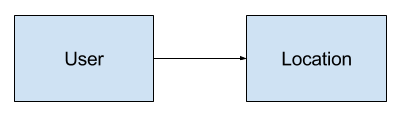
\includegraphics[width=1\linewidth]{img/join-simple.png}
\end{figure}

\end{frame}

\begin{frame}[fragile]{Simple join of a single relationship}

\begin{lstlisting}
my $rs = $schema->resultset('User')->search(
    undef,
    {
        join => 'locations',
    }
);
\end{lstlisting}
\end{frame}

Join several relationships:

\begin{frame}[fragile]{Join several relationships}
\begin{figure}[!ht]
\centering
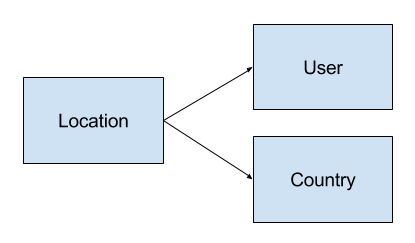
\includegraphics[width=1\linewidth]{img/join-several.png}
\end{figure}
\end{frame}

\begin{frame}[fragile]{Join several relationships}

\begin{lstlisting}
my $rs = $schema->resultset('Location')->search(
    undef,
    {
        join => [ 'user', 'country' ],
    }
);
\end{lstlisting}
\end{frame}

Multi-level join:

\begin{frame}[fragile]{Multi-level Join}
\begin{figure}[!ht]
\centering
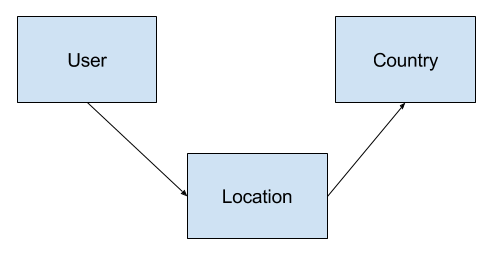
\includegraphics[width=1\linewidth]{img/join-multi-level.png}
\end{figure}
\end{frame}

\begin{frame}[fragile]{Multi-level Join}
\begin{lstlisting}
my $rs = $schema->resultset('User')->search(
    undef,
    {
        join => { locations => 'country' }
    }
);
\end{lstlisting}
\end{frame}

\begin{frame}[fragile]{Join}
\begin{figure}[!ht]
\centering
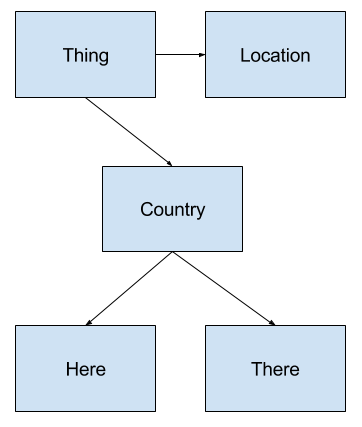
\includegraphics[width=0.4\linewidth]{img/join-complex.png}
\end{figure}
\end{frame}

\begin{frame}[fragile]{Join}
Several relationships combined with multi-level:

\begin{lstlisting}
    join => [
        'locations', { country => [ 'here', 'there' ] }
    ]
\end{lstlisting}
\end{frame}

join: Table aliases

DBIx::Class uses the relation names as table aliases. This is important when
you need to add grouping or ordering to your queries and also when
specifying column names in search conditions. It is essential if any of your
tables have columns with the same names. The source table is given the
default alias 'me'.

\begin{frame}[fragile]{Table aliases}
\begin{lstlisting}
my $rs = $schema->resultset('Country')->search(
    {
        'me.country_iso_code' => 'MT',
        'locations.city'      => 'Qormi',
    },
    {
        join => 'locations',
    }
);
\end{lstlisting}
\end{frame}

\begin{frame}[fragile]{Joining to the same table twice}

There is no magic to this, just do it. The table aliases will automatically
be numbered:

\begin{lstlisting}
join => [ 'room', 'room', 'room' ]
\end{lstlisting}

The aliases are: room, room\_2 and room\_3.
\end{frame}

\begin{frame}[fragile]{alias}
Value: \$source\_alias

    alias => 'table\_alias'

\end{frame}

Sometimes you need to be able to override the default source table alias especially for nested search queries (sub-SELECTs) and correlated subqueries. These will be covered in a later section.

\subsubsection{Columns returned}
\begin{frame}[fragile]{columns}

Restrict the list of columns to be returned:

\begin{lstlisting}
Value: \@columns | \%columns | $column
\end{lstlisting}

Array reference:

\begin{lstlisting}
my $rs = $schema->resultset('User')->search(
    undef,
    {
        columns => [qw/ username first_name last_name /],
    }
);
\end{lstlisting}
\end{frame}

\begin{frame}[fragile]{columns}

An equivalent result can be obtained using the select attribute:
\begin{lstlisting}
my $rs = $schema->resultset('User')->search(
    undef,
    {
        select => [qw/ username first_name last_name /],
    }
);
\end{lstlisting}
\end{frame}

\begin{frame}[fragile]{columns}

Hash reference:

\begin{lstlisting}
my $rs = $schema->resultset('User')->search(
    undef,
    {
        columns => {
            firstname => 'first_name',
            lastname => 'last_name',
        }
    }
);
\end{lstlisting}
\end{frame}

If the alias used (firstname/lastname in the example) does not correspond to
an existing column then it must be accessed via:

\begin{lstlisting}
$user->get_column('firstname');
\end{lstlisting}

Extra accessors can also be added - to be covered later.

An equivalent result can be obtained using the select and as attributes:

\begin{frame}[fragile]{columns}
\begin{lstlisting}
my $rs = $schema->resultset('User')->search(
    undef,
    {
        select => [ 'first_name', 'last_name' ],
        as     => [ 'firstname', 'lastname' ],
    }
);
\end{lstlisting}
\end{frame}

NOTE: columns is generally preferred to select and as since it is much
easier to read the intent from the code.

\begin{frame}[fragile]{columns}
Simple scalar:

\begin{lstlisting}
my $rs = $schema->resultset('User')->search(
    undef,
    {
        columns => 'first_name'
    }
);
\end{lstlisting}

\end{frame}

\begin{frame}[fragile]{columns}
Array reference with hash references:

\begin{lstlisting}
my $rs = $schema->resultset('User')->search(
    undef,
    {
        columns => [ 'username', { name => 'first_name' } ],
    }
);
\end{lstlisting}
\end{frame}

columns: Using database functions or stored procedures

\begin{frame}[fragile]{columns: Using database functions or stored
    procedures}
\begin{lstlisting}
my $rs = $schema->resultset('User')->search(
    {},
    {
        columns => [
            'username',
            { username_length => 
                { length => 'username' } }
        ],
    }
);
\end{lstlisting}
\end{frame}

+columns

\begin{frame}[fragile]{+columns}

Works the same as columns but adds columns to the current selection.

\begin{lstlisting}
my $rs = $schema->resultset('User')->search(
    undef,
    {
        join => 'locations',
        '+columns' => [ 'locations.country_iso_code' ]
    }
);
\end{lstlisting}
\end{frame}

NOTE: must be quoted even when used on the left hand side of a 'fat comma'.

In addition to +columns there are also +select and +as attributes which
operate much like select and as except they are for adding columns. It is
generally preferred to use +columns. The following are equivalent:

\begin{frame}[fragile]{Equivalent of +columns with +select and +as}
\begin{lstlisting}
my $rs = $schema->resultset('User')->search(undef,
    {
        join => 'locations',
        '+columns' => [ { code => 'locations.country_iso_code' } ]
    }
);

my $rs = $schema->resultset('User')->search(undef,
    {
        join => 'locations',
        '+select' => [ 'locations.country_iso_code' ],
        '+as'     => [ 'code' ],
    }
);
\end{lstlisting}
\end{frame}

\subsubsection{collapse}

Value: [ 0 | 1 ] - defaults to 0

When set to a true value, indicates that any rows fetched from joined
has\_many relationships are to be aggregated into the corresponding "parent"
object. For example:

\begin{frame}[fragile]{collapse}
\begin{lstlisting}
my $rs = $schema->resultset('User')->search(
    undef,
    {
        join       => 'locations',
        '+columns' => [ 'locations.country_iso_code' ],
    }
);
\end{lstlisting}
\end{frame}

This will return as many row objects as there locations since User has\_many
locations.

Compare with:

\begin{frame}[fragile]{collapse}
\begin{lstlisting}
my $rs = $schema->resultset('User')->search(
    undef,
    {
        join       => 'locations',
        '+columns' => [ 'locations.country_iso_code' ],
        collapse   => 1,
    }
);
\end{lstlisting}
\end{frame}

This will return only as many row objects as there are Users. The many locations related to each user are available via the locations accessor thus:

\begin{frame}[fragile]{collapse}
\begin{lstlisting}
while ( my $user = $rs->next ) {
    print "user " , $user->username ,
        " has the following country codes:\n";

    my $locations_rs = $user->locations;
    while ( my $location = $locations_rs->next ) {
        print "\t" , $location->country_iso_code , "\n";
    }
}
\end{lstlisting}
\end{frame}

\subsubsection{prefetch}

Value: \verb=$rel_name | \@rel_names | \%rel_names=

This attribute is a shorthand for specifying a join spec, adding all columns
from the joined related sources as +columns and setting collapse to a true
value. It can be thought of as a rough superset of join. Both join and
prefetch can be combined in a single search and DBIC will add columns
appropriately.

In the following query we join country in order to search by country name
but we do not include any columns from the country table in the
result. Using prefetch on locations means that all columns from the Location
class will be available via the locations accessor accessor for each user
object returned.

\begin{frame}[fragile]{prefetch}
\begin{lstlisting}
my $rs = $schema->resultset('User')->search(
    {
        'country.name' => 'Malta',
    },
    {
        join => { locations => 'country' },
        prefetch => 'locations',
    }
);
\end{lstlisting}
\end{frame}

This is equivalent to:

\begin{frame}[fragile]{prefetch}
\begin{lstlisting}
my $rs = $schema->resultset('User')->search(
{
    'country.name' => 'Malta',
},
{
    join => { locations => 'country' },
    '+columns' => [
        ( map { +{ "locations.$_" => "locations.$_" } }
              $schema->source('User')
                ->related_source('locations')->columns )
    ],
    collapse => 1,
}
);
\end{lstlisting}
\end{frame}

\subsubsection{order\_by}

Value: \verb=$order_by | \%order_by | \@order_by=

Which column(s) to order the results by. This can either be a scalar (just a
column name), a hash reference of \verb|{ -desc => 'col' }| or 
\verb|{ -asc => 'col' }|, or an array reference of either of the two
previous forms.

If a single column name, or an arrayref of names is supplied, the argument
is passed through directly to SQL. To ensure database-agnostic ordering the
hashref syntax should be used.

\begin{frame}[fragile]{order\_by}
\begin{table}
\begin{tabular}{l | l}
Given & Will Generate \\
\hline
\verb|'colA'| & ORDER BY colA \\ 
\verb|[ 'colA', 'colB' ]| & ORDER BY colA, colB \\
\verb|{ -asc => 'colA' }| & ORDER BY colA ASC \\
\verb|{ -desc => 'colB' }| & ORDER BY colB DESC \\
\verb|{ -asc => [ 'colA', 'colB' ] }| & ORDER BY colA ASC, colB ASC \\
\verb|{ -asc  => 'colA' }, { -desc => [ 'colB' ] }, { -asc  => [ 'colC', 'colD' ] }|
& ORDER BY colA ASC,
     colB DESC,
     colC ASC, colD ASC \\
\end{tabular}
\end{table}
\end{frame}

The old scalar reference syntax (i.e. \verb|order_by => \'year DESC'|) is
still supported, although you are strongly encouraged to use the hashref
syntax as outlined above.

\subsubsection{group\_by}

Value: \@columns

A arrayref of columns to group by. Can include columns of joined tables.

\begin{frame}[fragile]{group\_by}
\begin{lstlisting}
my $rs = $schema->resultset('User')->search(
    {},
    {
        columns    => 'username',
        '+columns' => [ 
            { country_name  => 'country.name' },
            { country_count => {
                count => 'country.country_iso_code' }
            },
        ],
        join => { locations => 'country' },
        group_by => [ 'me.username', 'country.name' ],
    },
);
\end{lstlisting}
\end{frame}

\subsubsection{page, rows and offset}

\verb|page| makes the resultset paged and specifies the page to
retrieve. Effectively identical to creating a non-paged resultset and then
calling \verb|->page($page)| on it.

If rows attribute is not specified it defaults to 10 rows per page.

NOTE: When you have a paged resultset, count will only return the number of
rows in the page. To get the total, use the pager and call total\_entries on
it. 

\verb|rows| specifies the maximum number of rows for direct retrieval, or
the number of rows per page if the page attribute or method is used.

\verb|offset|Specifies the (zero-based) row number for the first row to be
returned. If the resultset is paged then the offset is relative to the
current page.

\begin{frame}[fragile]{page, rows and offset}
Page 2 starts with the 6th row so this gives us rows 16 to 20:

\begin{lstlisting}
my $rs = $schema->resultset('Location')->search(
    {},
    {
        page   => 2,
        rows   => 5,
        offset => 10,
    }
);
\end{lstlisting}
\end{frame}

\subsection{Chaining}
% from riba's slides

\begin{frame}{Chaining}
  \begin{figure}[!ht]
    \begin{center}
      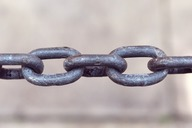
\includegraphics{img/chains.jpg}
      \caption[Chains]{Picture from Katrin Baustmann}
    \end{center}
  \end{figure}
\end{frame}

% picture from
% https://pixabay.com/en/chain-chain-link-border-demarcation-722278/
% Creative Commons CC0

\subsubsection{Shallow Nesting (Chaining)}

\begin{frame}[fragile]{Shallow Nesting (Chaining)}
\begin{lstlisting}
    $rs->search({ name => { '!=', 'blah' }})
        ->search({ name => { '!=', undef }})

    ... WHERE name != 'blah' AND name IS NOT null
\end{lstlisting}
\end{frame}

\subsubsection{Subquery nesting}

\begin{frame}[fragile]{Subquery nesting}
\begin{lstlisting}
    $rs->search({}, { distinct => 1 })
        ->as_subselect_rs
         ->search({}, { rows => 1 })

    ... SELECT FROM (SELECT * FROM artist GROUP_BY * )
        LIMIT 1
\end{lstlisting}
\end{frame}

\subsection{Correlated Subqueries}
\begin{frame}{Correlated Subqueries}
\end{frame}

\section{Relationships}

\begin{frame}{Relationships}
\begin{itemize}
\item has\_many, might\_have and has\_one
\item many\_to\_many
\item Relationship conditions
\item Relationship attributes
\item Relationships with nullable FKs
\end{itemize}
\end{frame}

\subsection{has\_many, might\_have and has\_one}

In DBIx::Class a relationship defines the connection between exactly two
tables. The relationship condition lists the columns in each table that
contain the same values. It is used to output an SQL JOIN condition between
the tables.

One side of the relationship is always a \verb|belongs_to| relationship
where the calling class stores the stores the foreign class’s primary key in
one (or more) of the calling class columns.

In our example schema every user can have zero, one or many locations and
each Location \verb|belongs_to| a single User so we have the following column and
relationship defined in the Location class: 
 
\begin{frame}[fragile]{belongs\_to}
\begin{lstlisting}
column users_id => {
    data_type      => "integer",
};

belongs_to
  user => "TravelDance::Schema::Result::User",
  { 'foreign.users_id' => 'self.users_id' };
\end{lstlisting}
\end{frame}

Here ‘user’ is the name of the relationship and also the name of the relationship accessor that is created. The second argument is the foreign class and the final argument is the relationship condition. Here we have a simple equality condition.

Note the use of ‘is\_foreign\_key’ in the users\_id column definition. This is used when the schema is deployed and instructs SQL::Translator to create the appropriate foreign key constraints in the database.

In the User class we define the primary key which is referenced by the Location class::

\begin{frame}[fragile]{Primary key}
\begin{lstlisting}
primary_column users_id => {
    data_type         => "integer",
    is_auto_increment => 1,
};
\end{lstlisting}
\end{frame}

And since we expect each user to have many locations we define the relationship as a \verb|has_many|:

\begin{frame}[fragile]{Locations Relationship}
\begin{lstlisting}
has_many locations =>
  "TravelDance::Schema::Result::Location",
  { 'foreign.users_id' => 'self.users_id' };
\end{lstlisting}
\end{frame}

Note: has\_many does not mean that there must be many related items but only that there can be many. One or zero related items is also possible (a LEFT JOIN).


\begin{frame}{has\_many / might\_have}
\begin{table}
\begin{tabular}{c | c | c}
relationship type & default join type & number of related rows \\
\hline
has\_many & LEFT & zero, one or many \\
might\_have & LEFT & zero or one \\
\end{tabular}
\end{table}
\end{frame}

The difference here is that with a collapsed search (to be covered later)
the has\_many accessor returns a resultset whereas the might\_have accessor
returns a result object (a single row).

\subsection{many\_to\_many}

This is not a relationship but a convenience method generator which defines an
accessor to retrieve row contents across multiple relationships.

The difference between a bridge and a relationship is, that the bridge
cannot be used to join tables in a search, instead its component
relationships must be used.

\subsection{Relationship conditions}

\begin{frame}{Relationship conditions}
\begin{itemize}
\item Simple equality
\item Multiple groups of simple equality conditions
\item Custom join conditions
\end{itemize}
\end{frame}

\subsubsection{Simple equality}

Simple equality conditions
in User:

\begin{frame}[fragile]{Simple equality conditions}
\begin{lstlisting}
has_many
  locations => "TravelDance::Schema::Result::Location",
  { 'foreign.users_id' => 'self.users_id' };
\end{lstlisting}
\end{frame}

If the column has the same name in both tables then the condition can be replaced with the column name:

\begin{frame}[fragile]{Simple equality conditions}
\begin{lstlisting}
has_many
  locations => "TravelDance::Schema::Result::Location",
  'users_id';
\end{lstlisting}
\end{frame}

\subsubsection{Multiple groups of simple equality conditions}

As is the default in SQL::Abstract, the key-value pairs will be ANDed in the
resulting JOIN clause. An OR can be achieved with an arrayref. For example a
condition like:

\begin{frame}[fragile]{Multiple groups of simple equality conditions}
\begin{lstlisting}
has_many
  related_item_links => "My::Schema::Item::Links",
  [
    { 'foreign.left_itemid'  => 'self.id' },
    { 'foreign.right_itemid' => 'self.id' },
  ];
\end{lstlisting}
\end{frame}

\subsubsection{Custom join conditions}

All locations visited before 1st January 2000.

\begin{frame}[fragile]{Custom join conditions}
\begin{lstlisting}
has_many
 before_2000 => "TravelDance::Schema::Result::Location",
 sub {
   my $args = shift;
   return {
      "$args->{foreign_alias}.users_id" =>
          { -ident => "$args->{self_alias}.users_id" },
      "$args->{foreign_alias}.visited" =>
          { '<', '2000-01-01' },
   };
 };
\end{lstlisting}
\end{frame}

\subsection{Relationship attributes}

% NOTE: we should mention these but not go into any detail except for join_type.

\begin{frame}{Relationship attributes}
\begin{itemize}
\item join\_type
% \item proxy => \verb|$column| | \verb|\@columns| | \verb|\%column|
\item accessor
\item is\_foreign\_key\_constraint
\item cascade\_copy / cascade\_delete / cascade\_update
\item on\_delete / on\_update
\item is\_deferrable
\item add\_fk\_index
\end{itemize}
\end{frame}

\subsection{Relationships with nullable FKs}

% Source for description: https://en.wikipedia.org/wiki/Marie_Byrd_Land
% License for Picture: CC BY 2.0 via Commons 

\subsubsection{Unclaimed Land}

Because of its remoteness, even by Antarctic standards, most of Marie Byrd
Land (the portion east of 150\degree{}W) has not been claimed by any sovereign
nation. It is by far the largest single unclaimed territory on Earth, with
an area of 1,610,000 km2 (620,000 sq mi) (including Eights Coast,
immediately east of Marie Byrd Land).

\begin{frame}{Unclaimed Land}
  \begin{figure}[!ht]
    \begin{center}
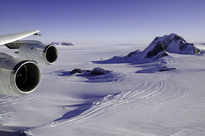
\includegraphics{img/Marie_Byrd_Land.jpg}
\caption[Marie Byrd Land]{Photo by Michael Studinger / NASA
  Goddard Space Flight Center}
    \end{center}
\end{figure}
\end{frame}

\subsubsection{Location without a country}

A location usually has a country but not if it is in a neutral zone like in
the middle of an ocean so this column is nullable:

\begin{frame}[fragile]{Location without a country}
\begin{lstlisting}
column country_iso_code => {
    data_type      => "char",
    size           => 2,
    is_nullable    => 1,
};
\end{lstlisting}
\end{frame}

Location has a belongs\_to relationship with Country and the default join
type for this relationship is an INNER JOIN (the default JOIN type) which
skips rows from the left-hand table if there is no corresponding row in the
right-hand table. Compare these two SQL queries and their result: 

\begin{frame}[fragile]{SQL queries}
\begin{lstlisting}
SELECT count(*) FROM locations l JOIN countries c
    ON l.country_iso_code=c.country_iso_code;
27

SELECT count(*) FROM locations l LEFT JOIN countries c
    ON l.country_iso_code=c.country_iso_code;
28
\end{lstlisting}
\end{frame}

So we use the join\_type relationship attribute in the relationship definition to force a LEFT JOIN:

\begin{frame}[fragile]{LEFT JOIN join\_type}
\begin{lstlisting}
belongs_to
  country => "TravelDance::Schema::Result::Country",
  "country_iso_code",
  { join_type => 'left' };
\end{lstlisting}
\end{frame}

\section{Extending Schema}
\begin{frame}{Extending Schema}
\begin{itemize}
\item Components
\item Helpers
\end{itemize}
\end{frame}

\subsection{Components}
DBIx::Class uses \href{https://metacpan.org/pod/Class::C3::Componentised}
{Class::C3::Componentised} to allow mix-ins (components) to be added to the 
various classes that together comprise the schema definition. 

There are three different kinds of components:

\begin{frame}{Component Types}
\begin{itemize}
\item \emph{Schema} class components
\item \emph{Result} class components
\item \emph{ResultSet} class components
\end{itemize}
\end{frame}
 
Many components exist for all of these three kinds.

\subsubsection{Schema Components}

Loading a component to your main Schema class:

\begin{frame}[fragile]{Schema Components}
\begin{lstlisting}
package TravelDance::Schema;
 
__PACKAGE__->load_components(
    'Helper::Schema::QuoteNames'
);
\end{lstlisting}
\end{frame}

\subsubsection{Using Result Class Components}

In a single result class:

\begin{frame}[fragile]{Using Components}
\begin{lstlisting}
package TravelDance::Schema::Result::User;

use TravelDance::Schema::Candy -components => [qw(
    InflateColumn::DateTime 
    PassphraseColumn
    TimeStamp
)];
\end{lstlisting}
\end{frame}

In order to add a result class component to \emph{all} result classes you
can add these to the list 
in \verb|TravelDance::Schema::Candy|'s \verb|parse_arguments|.

\paragraph{Password/passphrase columns}

DBIx::Class::PassphraseColumn uses the column definition when hashing a new
password/passphrase but can test the password against many types of hash
stored in the column. This allows an application to switch from (say)
MD5 crypt to blowfish whilst still working with the old hashes.

\begin{frame}[fragile]{Password column}
\begin{lstlisting}
column password => {
    data_type        => "text",
    default_value    => "",
    passphrase       => 'crypt',
    passphrase_class => 'BlowfishCrypt',
    passphrase_args  => {
        cost        => 14,
        key_nul     => 1,
        salt_random => 1,
    },
    passphrase_check_method => 'check_password',
};
\end{lstlisting}
\end{frame}

\paragraph{Automatic setting of date/datetime columns on create/update}
DBIx::Class::TimeStamp

From User class:

\begin{frame}[fragile]{Create/update date columns}
\begin{lstlisting}
column created => {
    data_type     => "datetime",
    set_on_create => 1,
};


column last_modified => {
    data_type     => "datetime",
    set_on_create => 1,
    set_on_update => 1,
};
\end{lstlisting}
\end{frame}

\subsubsection{Automatic DateTime inflation from columns}

Using DBIx::Class::InflateColumn::DateTime we can have date and datetime
columns automatically converted to DateTime objects when retrieved from the
database. The reverse also happens and DateTime objects are converted back
into a format appropriate for the underlying database engine on
create/update.

NOTE: Don't rely on InflateColumn::DateTime to parse date strings for
you. The column is set directly for any non-references and
InflateColumn::DateTime is completely bypassed. For example if you pass a
string value date directly to create/update then this will be stored AS IS
and on retrieve might be in a format that InflateColumn::DateTime’s inflator
does not understand resulting in an exception rather than the DateTime
object you are expecting. The rule is \verb|always| pass DateTime objects when
creating/updating a column with this inflator in place.

\subsubsection{ResultSet Components}

In order to be able to add a component to all ResultSet classes we need to
do:

\begin{frame}[fragile]{ResultSet Components}
\begin{itemize}
\item create parent class \\
  \verb|TravelDance::Schema::ResultSet|
\item set as default resultset class \\
  \verb|TravelDance::Schema|
\item use for custom resultset classes \\
 \verb|TravelDance::Schema::ResultSet::User|
\end{itemize}
\end{frame}

\paragraph{Create Parent Class}

\begin{frame}[fragile]{Create Parent Class}
\begin{lstlisting}
package TravelDance::Schema::ResultSet;

use base 'DBIx::Class::ResultSet';

__PACKAGE__->load_components("TimeStamp");
\end{lstlisting}
\end{frame}

\paragraph{Set as Default Resultset Class}

\begin{frame}[fragile]{Set as Default Resultset Class}
\begin{lstlisting}
package TravelDance::Schema;

__PACKAGE__->load_namespaces(
    default_resultset_class => 'ResultSet'
);

\end{lstlisting}
\end{frame}

\paragraph{Inherit from Parent Class}
\begin{frame}[fragile]{Inherit from Parent Class}
\begin{lstlisting}
package TravelDance::Schema::ResultSet::User;

use base 'TravelDance::Schema::ResultSet';

__PACKAGE__->load_components(
    qw(Helper::ResultSet::CorrelateRelationship)
);
\end{lstlisting}
\end{frame}

\subsection{DBIx::Class Helpers}

\begin{frame}{CorrelateRelationship}

Problem: we want a count of rows in a related table

\end{frame}

So the obvious approach for this is:

\begin{frame}[fragile]{CorrelateRelationship}
\begin{lstlisting}
    my $rs = $schema->resultset('Author')->search(
        undef,
        {
            join       => 'books',
            '+columns' => {
                book_count => {
                    count => 'books.id'
                }
            },
            distinct   => 1,    # let DBIC work out group_by for us
        }
    );
\end{lstlisting}
\end{frame}
This causes a number of problems:

\begin{itemize}
\item Depending on engine, COUNT’s that aren’t COUNT(*) tend to be slow as
they do table scans.
\item This is hard to chain since we've introduced JOIN and GROUP BY and
collapsed COUNTs might produced unexpected results.
\item We cannot add other interesting data from the locations in the same query (such as date of most recent visit).
\end{itemize}

\begin{frame}[fragile]{CorrelateRelationship}
\begin{lstlisting}
Much nicer to do:

    package MyApp::Schema::ResultSet::Author;

    use parent 'DBIx::Class::ResultSet';

   
__PACKAGE__->load_components(qw(Helper::ResultSet::CorrelateRelationship));

    sub with_book_count {
        my $self = shift;

        $self->search(
            undef,
            {
                '+columns' => {
                    book_count =>
$self->correlate('books')->count_rs->as_query
                }
            }
        );
    }
\end{lstlisting}
\end{frame}

\begin{frame}[fragile]{CorrelateRelationship}
Then elsewhere:

\begin{lstlisting}
my $rs = $schema->resultset('Author')->with_book_count;

The SQL query will look something like this:

  SELECT me.id, me.name, me.foo, ..., (
    SELECT COUNT( * )
      FROM books books_alias
     WHERE books_alias.id = authors.id
   )
  FROM authors me

This is *much* faster and *always* chainable since no JOIN, GROUP BY, or
other junk added to query.
\end{lstlisting}
\end{frame}

Cool example from Interchange6::Schema::ResultSet::Product :

\begin{lstlisting}
    sub with_average_rating {
        my $self = shift;

        return $self->search(
            undef,
            {
                '+select' => [
                    {
                        coalesce => [

                            $self->correlate('canonical')
                              ->related_resultset('_product_reviews')
                              ->search_related(
                                'message',
                                { 'message.approved' => 1,
'message.public' => 1 }
                             
)->get_column('rating')->func_rs('avg')->as_query,

                            $self->correlate('_product_reviews')
                              ->search_related(
                                'message',
                                { 'message.approved' => 1,
'message.public' => 1 }
                             
)->get_column('rating')->func_rs('avg')->as_query,

                          ],
                        -as => 'average_rating'
                    }
                ],
                '+as' => ['average_rating'],
            }
        );
    }
\end{lstlisting}

\subsubsection{Helper::Resultset::Me}

Predefined queries present a problem: what is the table alias I need to use?
We can do:

\begin{frame}[fragile]{Helper::Resultset::Me}
\begin{lstlisting}
sub in_germany {
    my $self = shift;
    my $current_source_alias =
        $self->current_source_alias;
    return $self->search(
        { "$current_source_alias.country_iso_code"
          => 'DE' }
    );
}
\end{lstlisting}
\end{frame}

but using this helper makes things much simpler:

\begin{frame}[fragile]{Helper::Resultset::Me}
\begin{lstlisting}
sub in_germany {
    my $self = shift;


    return $self->search(
        { $self->me('country_iso_code') => 'DE' }
    );

}
\end{lstlisting}
\end{frame}

\subsubsection{Helper::Resultset::Random}

We use this in Interchange6 for finding random 'similar products' and other
such searches.

Three random countries:

\begin{frame}[fragile]{Helper::Resultset::Me}
\begin{lstlisting}

my $countries = $schema->resultset('Country')->rand(3);

\end{lstlisting}
\end{frame}

\subsubsection{Helper::ResultSet::RemoveColumns}
Have a result class with a large number of columns and you want all except
one (or more) of them:

\begin{frame}[fragile]{Helper::ResultSet::RemoveColumns}
\begin{lstlisting}
my $rs = $schema->resultset('User')->search(
    undef,
    {
        remove_columns => [ 'password' ],
    }
);
\end{lstlisting}
\end{frame}

Make that the default for searches (though this is not generally recommended):

\begin{frame}[fragile]{Helper::ResultSet::RemoveColumns}
\begin{lstlisting}
package TravelDance::Schema::Result::User;

__PACKAGE__->resultset_attributes(
    { remove_columns => [ 'password' ] }
);
\end{lstlisting}
\end{frame}

\subsubsection{Helper::ResultSet::Shortcut}

\begin{frame}[fragile]{distinct Shortcut}

\verb|distinct| shortcut:

\begin{lstlisting}
$rs->distinct;
\end{lstlisting}

equivalent to:

\begin{lstlisting}
$rs->search(undef, { distinct => 1 });
\end{lstlisting}
\end{frame}

\begin{frame}[fragile]{group\_by Shortcut}

\verb|group\_by| shortcut:

\begin{lstlisting}
$rs->group_by([ qw/ some column names / ]);
\end{lstlisting}

equivalent to:

\begin{lstlisting}
$rs->search(undef, { 
    group_by([ qw/ some column names / ] 
});
\end{lstlisting}
\end{frame}

\begin{frame}[fragile]{order\_by Shortcut}

\verb|order_by| Shortcut:

\begin{lstlisting}
$rs->order_by({ -desc => 'col1' });
\end{lstlisting}

equivalent to:

\begin{lstlisting}
$rs->search(undef, { order_by => { -desc => 'col1' });
\end{lstlisting}

\end{frame}

\begin{frame}[fragile]{order\_by Shortcut}

Funky magic stuff:
\begin{lstlisting}
$rs->order_by('!col1')
# { order_by => { -desc => 'col1' } }

$rs->order_by('col1,col2')
# { order_by => [{ -asc => 'col1' },{ -asc => 'col2' }]}

$rs->order_by('col1,!col2')
# { order_by => [{ -asc => 'col1' },{ -desc => 'col2' }]}
\end{lstlisting}
\end{frame}

\begin{frame}[fragile]{hri Shortcut}

\verb|hri| shortcut:

\begin{lstlisting}
$rs->hri;
\end{lstlisting}

equivalent to:

\begin{lstlisting}
$rs->search( undef, {
    result_class => 
        'DBIx::Class::ResultClass::HashRefInflator'
});
\end{lstlisting}
\end{frame}

\begin{frame}[fragile]{page Shortcut}

\verb|page| shortcut:

\begin{lstlisting}
$rs->page(2);
\end{lstlisting}

equivalent to:

\begin{lstlisting}
$rs->search( undef, { page => 2 } );
\end{lstlisting}

\end{frame}

rows / limit

\begin{frame}[fragile]{rows / limit Shortcut}

\begin{lstlisting}
$rs->rows(3);
\end{lstlisting}

or:

\begin{lstlisting}
$rs->limit(3);
\end{lstlisting}

equivalent to:

\begin{lstlisting}
$rs->search( undef, { rows => 3 } );
\end{lstlisting}

\end{frame}

\begin{frame}[fragile]{limited\_page Shortcut}

\verb|limited_page| shortcut:

\begin{lstlisting}
$rs->limited_page( 2, 3 );
\end{lstlisting}

equivalent to:

\begin{lstlisting}
$rs->search( undef, { page => 2, rows => 3 } );
\end{lstlisting}

\end{frame}

\begin{frame}[fragile]{has\_rows Shortcut}

A lighter way to check if the resultset has data compared to using count.

\begin{lstlisting}
$rs->has_rows;
\end{lstlisting}

equivalent to:

\begin{lstlisting}
$rs->search( undef, { rows => 1 } )->next;
\end{lstlisting}
\end{frame}

results\_exists:

\begin{frame}[fragile]{results\_exists Shortcut}

An alternative way to check if the resultset has data using the EXISTS SQL function. Possibly lighter-weight than using count.

\begin{lstlisting}
$rs->search(...)->results_exist
\end{lstlisting}
\end{frame}

\begin{frame}[fragile]{columns Shortcut}

\verb|columns| shortcut:

\begin{lstlisting}
$rs->columns([qw/ first_name last_name /]);
\end{lstlisting}

equivalent to:

\begin{lstlisting}
$rs->search( undef, { 
    columns => [qw/ first_name last_name /] 
} );
\end{lstlisting}

\end{frame}

\begin{frame}[fragile]{add\_columns Shortcut}

\verb|add_columns| shortcut:

\begin{lstlisting}
$rs->add_columns([qw/ some column names /]);
\end{lstlisting}

equivalent to:

\begin{lstlisting}
$rs->search( undef,
    { '+columns' => [qw/ some columns names /] }
);
\end{lstlisting}
\end{frame}

\begin{frame}[fragile]{prefetch Shortcut}

\verb|prefetch| shortcut:

\begin{lstlisting}
$rs->prefetch( { locations => 'country' } );
\end{lstlisting}

equivalent to:

\begin{lstlisting}
$rs->search( undef, { 
    prefetch => { locations => 'country' } 
} );
\end{lstlisting}

\end{frame}

% null ( @columns || \@columns )

\begin{frame}[fragile]{null Shortcut}

\verb|null| shortcut:

\begin{lstlisting}
$rs->null( 'col1', 'col2' );
\end{lstlisting}

or:

\begin{lstlisting}
$rs->null([ 'col1', 'col2' ]);
\end{lstlisting}

equivalent to:

\begin{lstlisting}
$rs->search({ col1 => undef, col2 => undef });
\end{lstlisting}
\end{frame}

%not\_null ( @columns || \@columns )

\begin{frame}[fragile]{not\_null Shortcut}

\verb|not_null| shortcut:

\begin{lstlisting}
$rs->not_null( 'col1', 'col2' );
\end{lstlisting}

or:

\begin{lstlisting}
$rs->not_null([ 'col1', 'col2' ]);
\end{lstlisting}

equivalent to:

\begin{lstlisting}
$rs->search({
    col1 => { '!=' => undef }, col2 => { '!=' => undef }
});
\end{lstlisting}
\end{frame}

%like ( @columns || \@columns, $cond )

\begin{frame}[fragile]{like Shortcut}

\verb|like| shortcut:

\begin{lstlisting}
$rs->like( 'city', 'region', '%York' );
\end{lstlisting}

or:

\begin{lstlisting}
$rs->like([ 'city', 'region' ], '%York' );
\end{lstlisting}

equivalent to:

\begin{lstlisting}
$rs->search(
    { city => { -like => '%York' },
    { region => { -like => '%York' },
);
\end{lstlisting}
\end{frame}

% not\_like ( @columns || \@columns, $cond )

\begin{frame}[fragile]{not\_like Shortcut}

\verb|not_like| shortcut:

\begin{lstlisting}
$rs->not_like( 'city', 'region', '%York' );
\end{lstlisting}

or:

\begin{lstlisting}
$rs->not_like([ 'city', 'region' ], '%York' );
\end{lstlisting}

equivalent to:

\begin{lstlisting}
$rs->search(
    { city => { -not_like => '%York' },
    { region => { -not_like => '%York' },
);

\end{lstlisting}
\end{frame}

\subsubsection{Helper::Row::NumifyGet}

\begin{frame}[fragile]{Helper::Row::NumifyGet}

Force numeric context on numeric columns:

\begin{lstlisting}
package TravelDance::Schema::Result::Foo_Bar;

use TravelDance::Schema::Candy -components =>
    [qw(Helper::Row::NumifyGet)];

column foo => {
    data_type   => 'integer',
    is_nullable => 0,
    is_numeric  => 1,   # the magic key
};
\end{lstlisting}
\end{frame}

\begin{frame}[fragile]{Helper::Row::NumifyGet}
\begin{lstlisting}
sub TO_JSON {
    return {
        # 0 instead of "0" due to context
        foo => $self->foo,  
    }
}
\end{lstlisting}
\end{frame}

\subsubsection{Helper::Row::OnColumnChange}

\begin{frame}[fragile]{Helper::Row::OnColumnChange}

Do things when the value of a column changes.

\begin{itemize}
\item before\_column\_change
\item around\_column\_change
\item after\_column\_change
\end{itemize}

\end{frame}

\begin{frame}[fragile]{Helper::Row::OnColumnChange}

\begin{lstlisting}
package TravelDance::Schema::Result::User;

use TravelDance::Schema::Candy -components =>
    [qw(Helper::Row::OnColumnChange 
        InflateColumn::DateTime)];

use DateTime;

column last_password_change => {
    data_type => timestamp,
};
\end{lstlisting}
\end{frame}

\begin{frame}[fragile]{Helper::Row::OnColumnChange}

On password change:

\begin{itemize}
\item check new password against old one
\item update \verb|last_password_change| column
\end{itemize}

\end{frame}

\begin{frame}[fragile]{Helper::Row::OnColumnChange}
\begin{lstlisting}
after_column_change password => {
    method   => 'change_password',
    txn_wrap => 1,  # wrap it all in a transaction
};
\end{lstlisting}
\end{frame}

\begin{frame}[fragile]{Helper::Row::OnColumnChange}
\begin{lstlisting}
sub change_password {
    my ( $self, $old_value, $new_value ) = @_;
    if ( $self->check_password($new_value) ) {
        $self->throw_exception("Password not changed")
    }
    else {
        $self->update(
            { last_password_change => DateTime->now() }
        );
    }
}
\end{lstlisting}
\end{frame}

\subsubsection{Helper::Schema::DateTime}

\begin{frame}[fragile]{Helper::Schema::DateTime}
Locations visited in the last year:

\begin{lstlisting}
my $one_year_ago = $schema->format_datetime(
    DateTime->now->subtract( year => 1 )
);

my $rs = $schema->resultset('Location')->search(
    {
        visited => { '>' => $one_year_ago }
    }
);
\end{lstlisting}
\end{frame}

\begin{frame}[fragile]{Helper::Schema::DateTime}

Without the helper:

\begin{lstlisting}
my $dtf = $schema->storage->datetime_parser; # boilerplate
my $one_year_ago = $dtf->format_datetime(
    DateTime->now->subtract( year => 1 )
);

my $rs = $schema->resultset('Location')->search(
    {
        visited => { '>' => $one_year_ago }
    }
);
\end{lstlisting}
\end{frame}

\subsubsection{Helper::QuoteNames}

\begin{frame}{Helper::QuoteNames}
This should always be used. Force quote\_names in your database
connect\_info so nobody can forget to add it later.
\end{frame}

Using the HashRefInflator makes sense when you need to quickly retrieve
data from a massive resultset or you need a list of hash references anyway,
e.g. for input to a template in a web application.

\begin{frame}[fragile]{HashRefInflator}
\begin{lstlisting}
my $rs = $schema->resultset('Country')->search({}, {
   result_class
     => 'DBIx::Class::ResultClass::HashRefInflator',
 });
\end{lstlisting}
\end{frame}

\begin{frame}[fragile]{HashRefInflator with HRI helper}
\begin{lstlisting}
my $rs = $schema->resultset('Country')->search({})->hri;

# since 'search' here is redundant we can just use:
my $rs = $schema->resultset('Country')->hri;
\end{lstlisting}
\end{frame}

% \section{Writing Tests}
% \begin{frame}{Writing Tests}
% \end{frame}

\section{Deployment Handler}

\subsection{Deploy/Upgrade/Downgrade}

\begin{frame}{Deployment Handler}
\begin{itemize}
\item DBIx::Class::DeploymentHandler
\item Deploy databases
\item Upgrade databases
\item Downgrade databases
\end{itemize}
\end{frame}

\subsection{Principles}

\begin{frame}{Principles}
\begin{itemize}
\item Create backup
\item Change schema
\item Add custom scripts
\item Bump version number
\item Prepare upgrade
\item Deploy upgrade
\end{itemize}
\end{frame}

Note: create backup can be done by DeploymentHandler itself.

\subsection{Change Schema}

\begin{frame}{Change Schema}
\begin{itemize}
\item Add table
\item Add column
\item Alter column
\end{itemize}
\end{frame}

\subsection{Bump version number}
\begin{frame}{Bump version number}
\begin{itemize}
\item Natural number => 1
\item Increase by 1 => 2
\end{itemize}
\end{frame}

\begin{frame}[fragile]{Version 1}
\begin{lstlisting}
package TravelDance::Schema;
use warnings;
use strict;
use base 'DBIx::Class::Schema';

our $VERSION = 1;

__PACKAGE__->load_namespaces();

1;
\end{lstlisting}
\end{frame}

\begin{frame}[fragile]{Version 2}
\begin{lstlisting}
package TravelDance::Schema;
use warnings;
use strict;
use base 'DBIx::Class::Schema';

our $VERSION = 2;

__PACKAGE__->load_namespaces();

1;
\end{lstlisting}
\end{frame}

\subsection{Prepare upgrade}

\begin{frame}[fragile]{Prepare upgrade}
\begin{lstlisting}
my $dh     = DBIx::Class::DeploymentHandler->new(
    {
        schema              => $schema,
        databases           => 'MySQL',
        sql_translator_args => { add_drop_table => 0 }
    }
);
$dh->prepare_deploy;
$dh->prepare_upgrade(
    {
        from_version => $dh->database_version,
        to_version => $dh->schema_version
    }
);
\end{lstlisting}
\end{frame}

\subsection{Add custom scripts}

\begin{frame}{Add custom scripts}
\begin{itemize}
\item Add initial values for new tables
\begin{itemize}
\item hardcoded in script
\item from file
\end{itemize}
\end{itemize}
\end{frame}

\subsection{Internals}

\begin{frame}{Directories and files}
\end{frame}

\end{document}

%%% Local Variables: 
%%% mode: latex
%%% TeX-master: t
%%% End: 
